\section{Présentation du sujet}

Mon stage est surtout lié à la suite de logiciel \gls{lc3d}, notamment celui de la piscine que j’avais à disposition.

Plusieurs problématiques interviennent vis-à-vis de l’implémentation existantes. En particulier, la “contrainte” la plus importante et que les utilisateurs concernés (piscinier, voiliste) n’ont aucune connaissance préalables en informatiques, et n’ont pour beaucoup jamais manipuler de logiciel.Cela nécessite que le logiciel soit simple et intuitif.
Les principaux inconvénient lié à cela sont les suivants :
\begin{itemize}
    \item Plus il y a d’action à réaliser, plus l’utilisateur risque de trouver cela compliqué: 
        \begin{itemize}
            \item L'utilisateur doit sélectionner quatres pixels dans un ordre correcte pour l'etape de calibration
            \item Il doit faire le masquage à la main s’il veut gérer les occlusion
            \item La prise de mesures réelle, nécessaire à la calibration, n’est pas toujours évidente.
            \item Si la mire utilisé et celle vendu par l’entreprise, alors les dimension sont connu , si non il faut que le clients les prennent lui même. En particulier pour la mire “fenêtre” il doit aussi spécifier la distance entre le sol et la mire.
        \end{itemize}
    \item Niveau technique, le plan relatif au sol généré, peut présenter quelques incohérences en fonction de la nature du terrain (Figure \ref{fig:problemsol}) 
\end{itemize}

\begin{figure}[!ht]
\centering
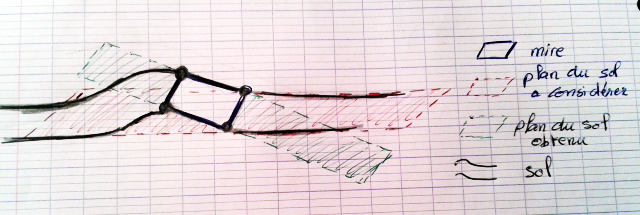
\includegraphics[width = 10cm] {images/croquisProblemeSol.jpg}
\caption{Illustration du problème de détéction du sol pouvant survenir à cause du terrain }
\label{fig:problemsol}
\end{figure}

L’objectif principal de mon stage consiste alors à simplifier et améliorer l’étape de calibration réalisé afin de permettre  de corriger ou limiter l’impact des contraintes cités.
\begin{itemize}
    \item En apportant des modification au code déjà existant
    \item En mettant en place de nouvelle méthodes de calibration
\end{itemize}

Mon sujet n’est pas alors constitué d'un projet défini à mettre en place et implémenter sur toute la durée du stage, mais de plusieurs pistes de solution à chercher et exploiter. L'intitulé de mon stage fait en fait partie d'une des piste envisagée qui semblait être dans un premier temps une solution idéale. J'expliquerai tout cela en détail dans la partie suivante.

